\documentclass{article}
\usepackage{amsmath,amsfonts,amssymb}
\usepackage{tikz,pgfplots}

\title{Solution}
\author{Shubham Tiwari}
\date{\today}

\begin{document}
\maketitle
\section*{Solution 1}
\[ \sum_{k=1}^{n} k = \frac{n(n+1)}{2} \]

\section*{Solution 2}
$\text{Positive numbers a,b, and c are the side lengths of a triangle if and only if} \\  a+b>c,b+c>a,c+a>b.$

\section*{Solution 3}
\[ \frac{d}{dx} \left (\frac{x}{x+1} \right) = \frac{1}{(x+1)^2}\]

\section*{Solution 4}
\begin{align*}
1+2 &= 3 \\
4+5+6 & = 7+8 \\
9+10+11+12 & = 13+14+15
\end{align*}

\section*{Solution 5}
\begin{center}
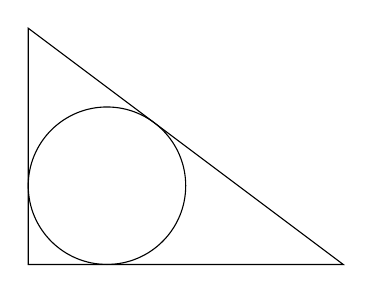
\begin{tikzpicture}
\draw (1,1) circle (1) ;
\draw (0,0) -- (0,3) -- (4,0) -- cycle ;
\end{tikzpicture}
\end{center}

\newpage
\begin{tikzpicture}
\draw (0,0) -- node[below]{6} (6,0) -- node[right]{5}(6,5) -- node[above left]{$\sqrt{61}$} cycle;
\draw (5.5,0) -- (6,0) -- (6,0.5) -- (5.5,0.5) -- cycle  ;


\end{tikzpicture}
\section{circle}
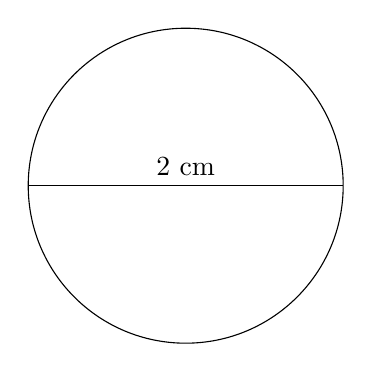
\begin{tikzpicture}
\draw (0,0) circle (2) ;
\draw (-2,0) -- node[above]{2 cm}(2,0);
\end{tikzpicture}

\section*{Plots}
\begin{tikzpicture}
\begin{axis}[axis lines = middle]
\addplot[domain=0:2]{sqrt(x)};
\addplot[domain=0:2,samples = 100]{x^2};
\end{axis}
\end{tikzpicture}



\end{document}